\subsection{Variances and Covariances}

\mode<presentation>{
\begin{frame} 
    \begin{center} \huge
        \subsecname
    \end{center}
    \begin{center}And knowing how to read contour plots
    \end{center}
\end{frame}
}

\begin{frame}\frametitle{\subsecname}

Let $\vec x \in \R^N$.

\begin{equation}
\text{Variance}~\sigma_j^2 = \E\Big\lbrack~(x_j - m_j)^2~\Big\rbrack = \frac{1}{p} \sum\limits_{\alpha = 1}^p 
		 \Big( \mathrm{x}_j^{(\alpha)} - m_j \Big)^2 \quad \forall j=1,\ldots,N
\end{equation}

\pause

\begin{equation}
	\text{Covariance matrix } \vec{C} = \big\{ C_{ij} \big\} \quad \text{with} \quad
	C_{ij} = \frac{1}{p} \sum\limits_{\alpha = 1}^p 
		 \Big( \mathrm{x}_i^{(\alpha)} - m_i \Big) 
		 \Big( \mathrm{x}_j^{(\alpha)} - m_j \Big)
\end{equation}

%\vspace{0.7cm}

\begin{equation}
C_{ii} = \sigma^2_i
\end{equation}

$\vec{C}_{N \times N}$ is real and symmetric.

		
\end{frame}

\definecolor{darkgreen}{rgb}{0,0.5,0}
\definecolor{byzantium}{rgb}{0.44, 0.16, 0.39}

\begin{frame}\frametitle{Covariance matrix}

\mode<presentation>{
\only<1>{
\begin{center}
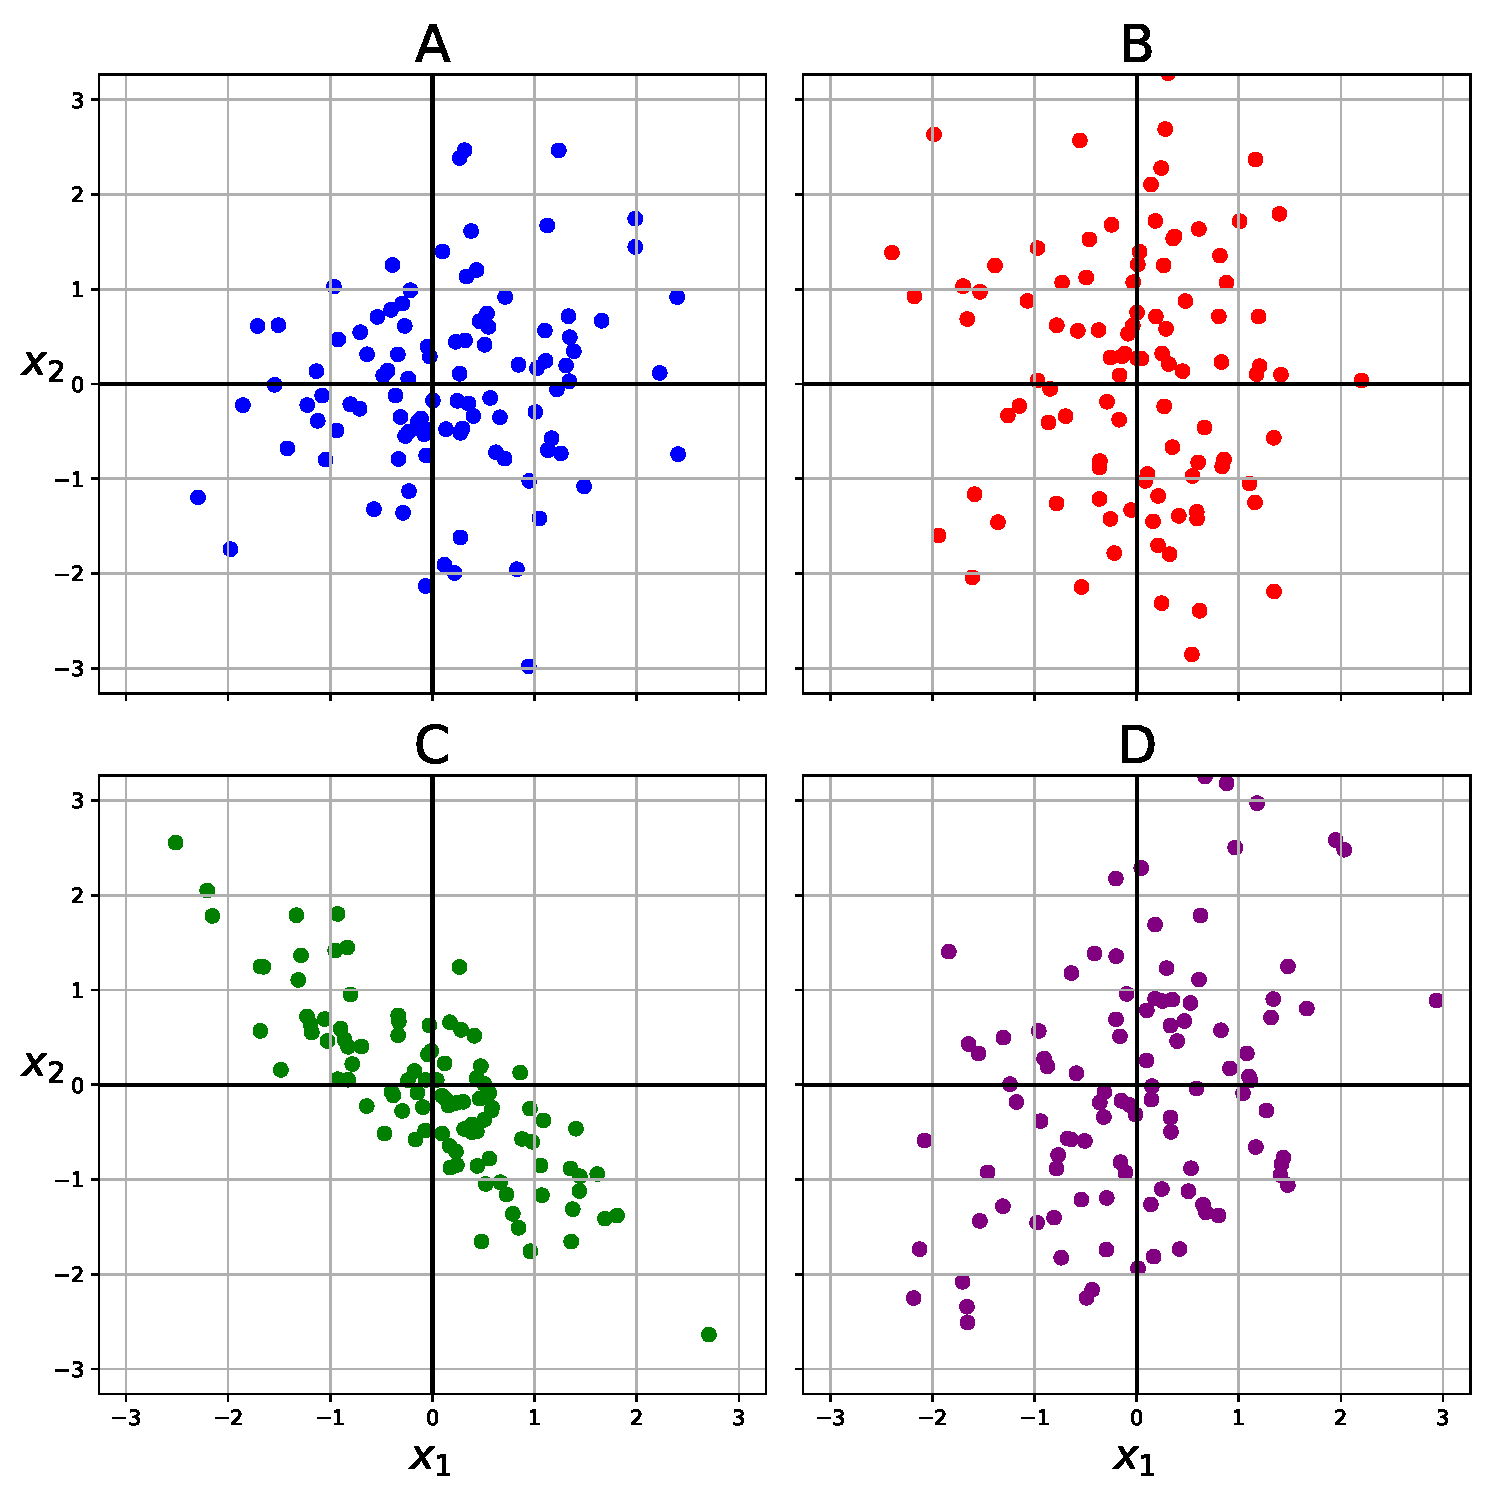
\includegraphics[width=0.6\textwidth]{img/scatter}%
\end{center}
}
\only<2>{
\begin{center}
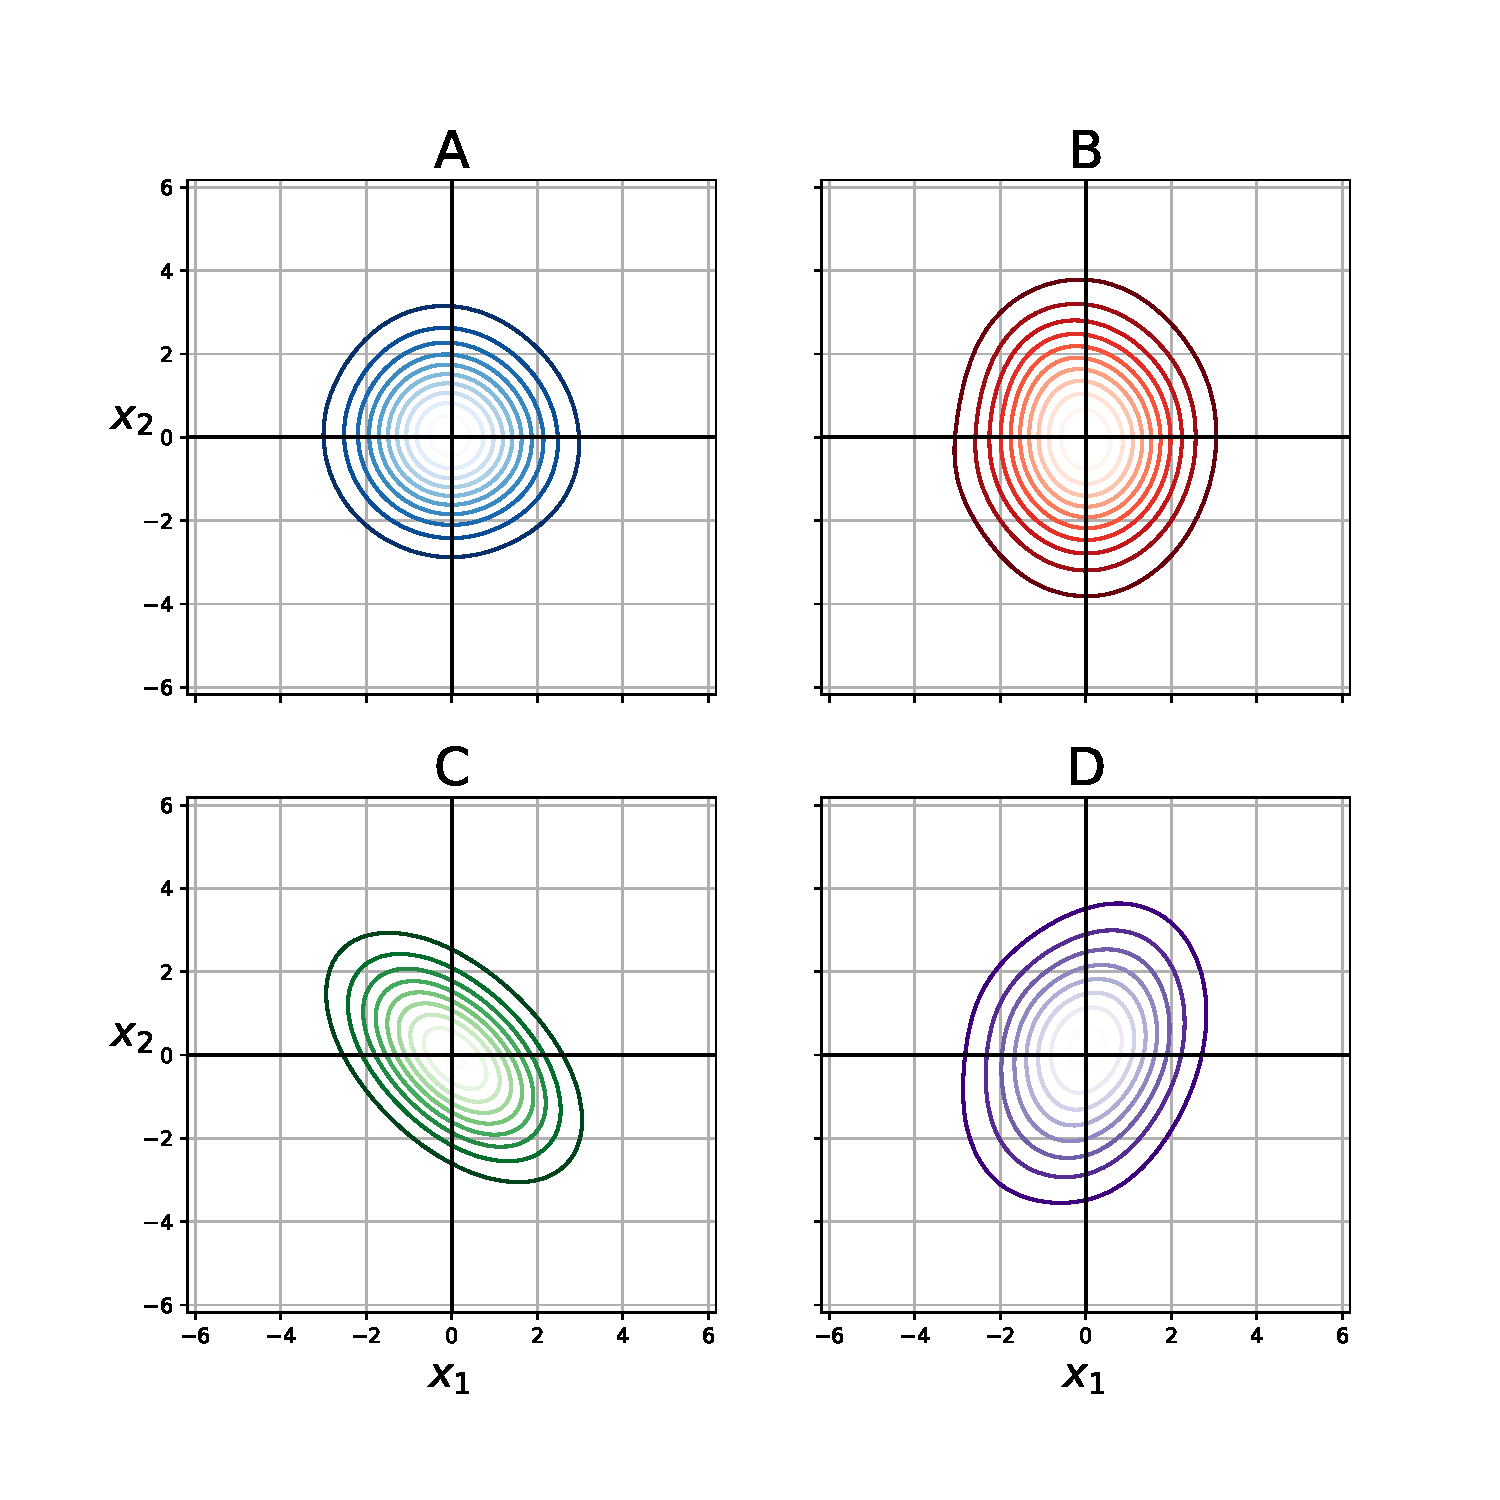
\includegraphics[width=0.6\textwidth]{img/cov}%
\end{center}

\slidesonly{\vspace{-10mm}}
}
}


\mode<article>{

\begin{figure}[ht]
     \centering
     \savebox{\imagebox}{
	 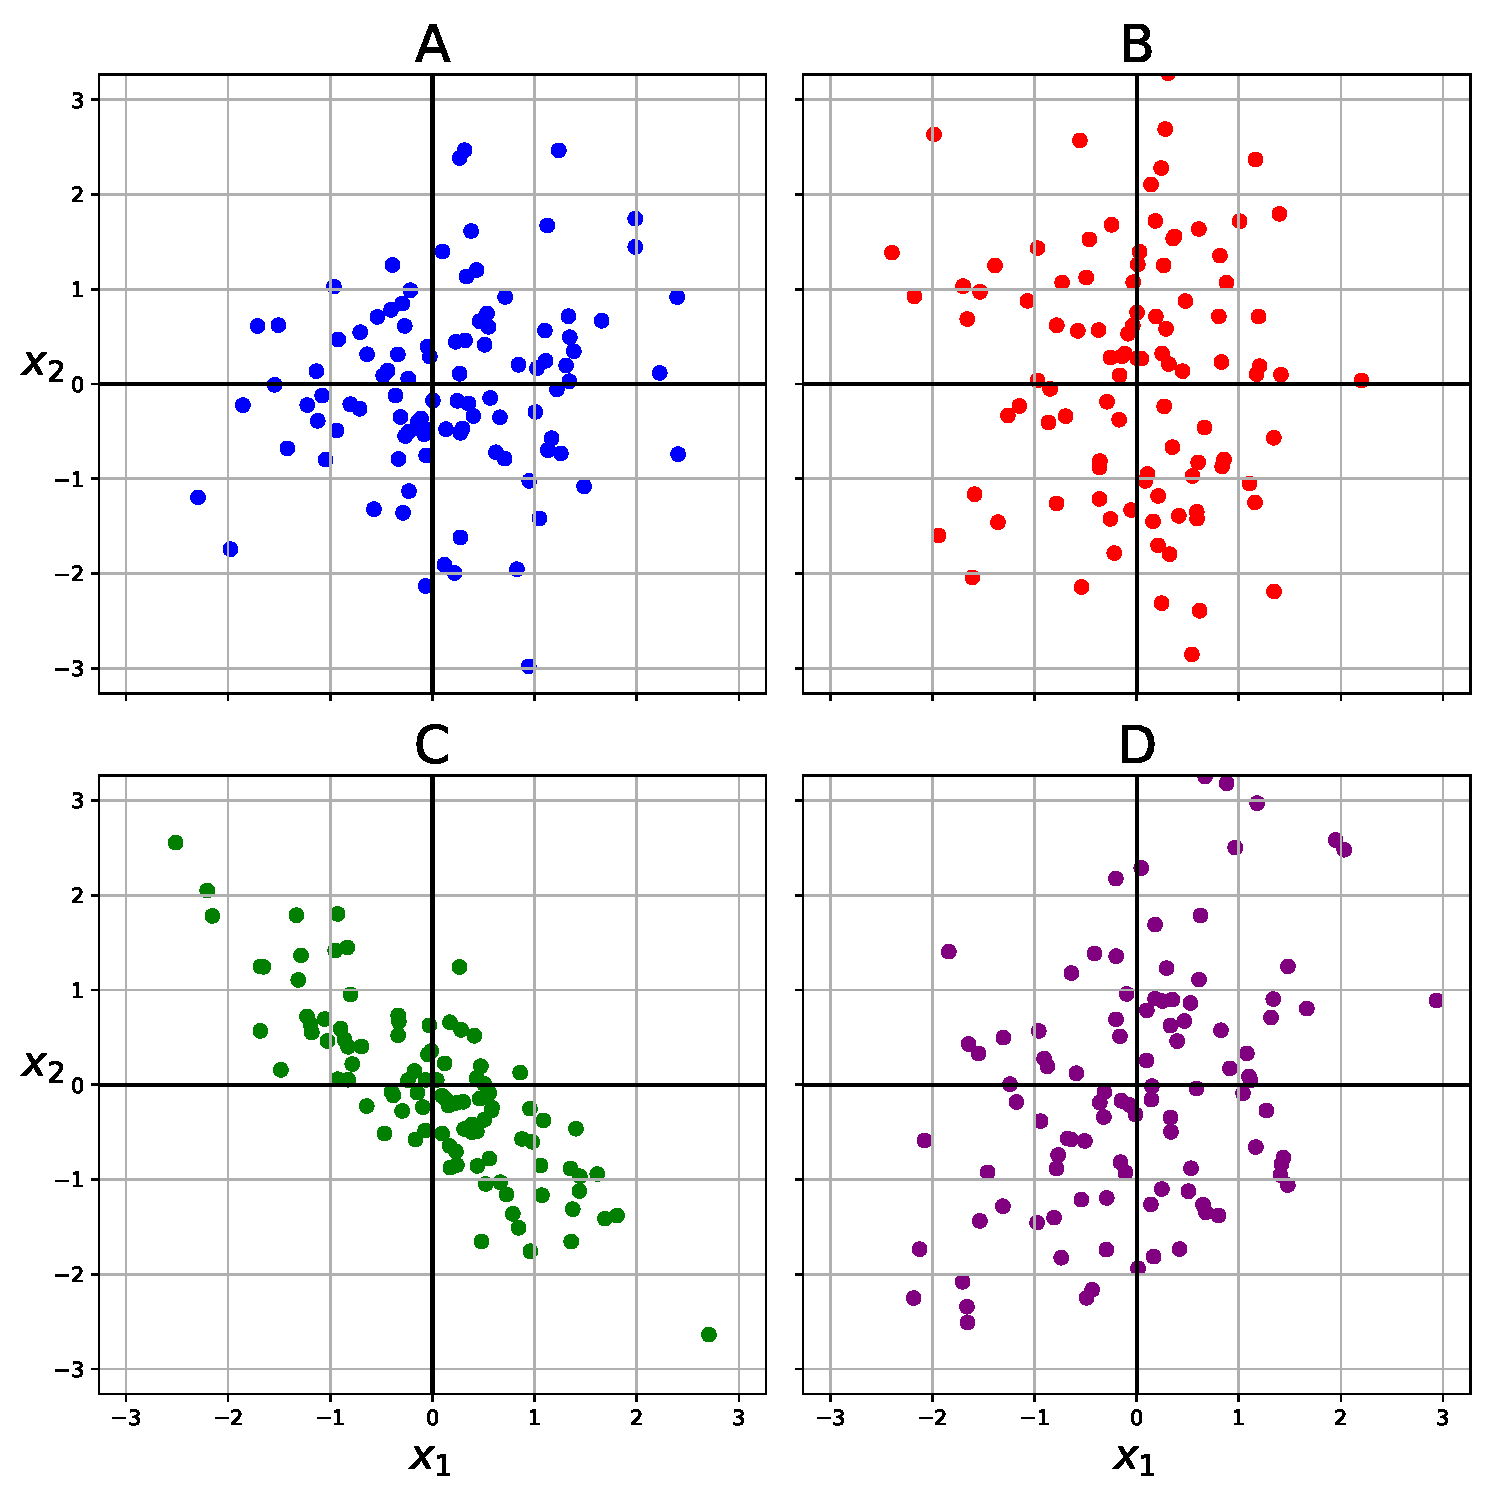
\includegraphics[width=0.33\textwidth]{img/scatter}}%
     \begin{subfigure}[t]{0.33\textwidth}
         \centering
         \usebox{\imagebox}% Place largest image
         \caption{Scatter plots}
     \end{subfigure}
     \hspace{2mm}
     \begin{subfigure}[t]{0.33\textwidth}
         \centering
         \raisebox{\dimexpr.5\ht\imagebox-.5\height}{% Raise smaller image into place
         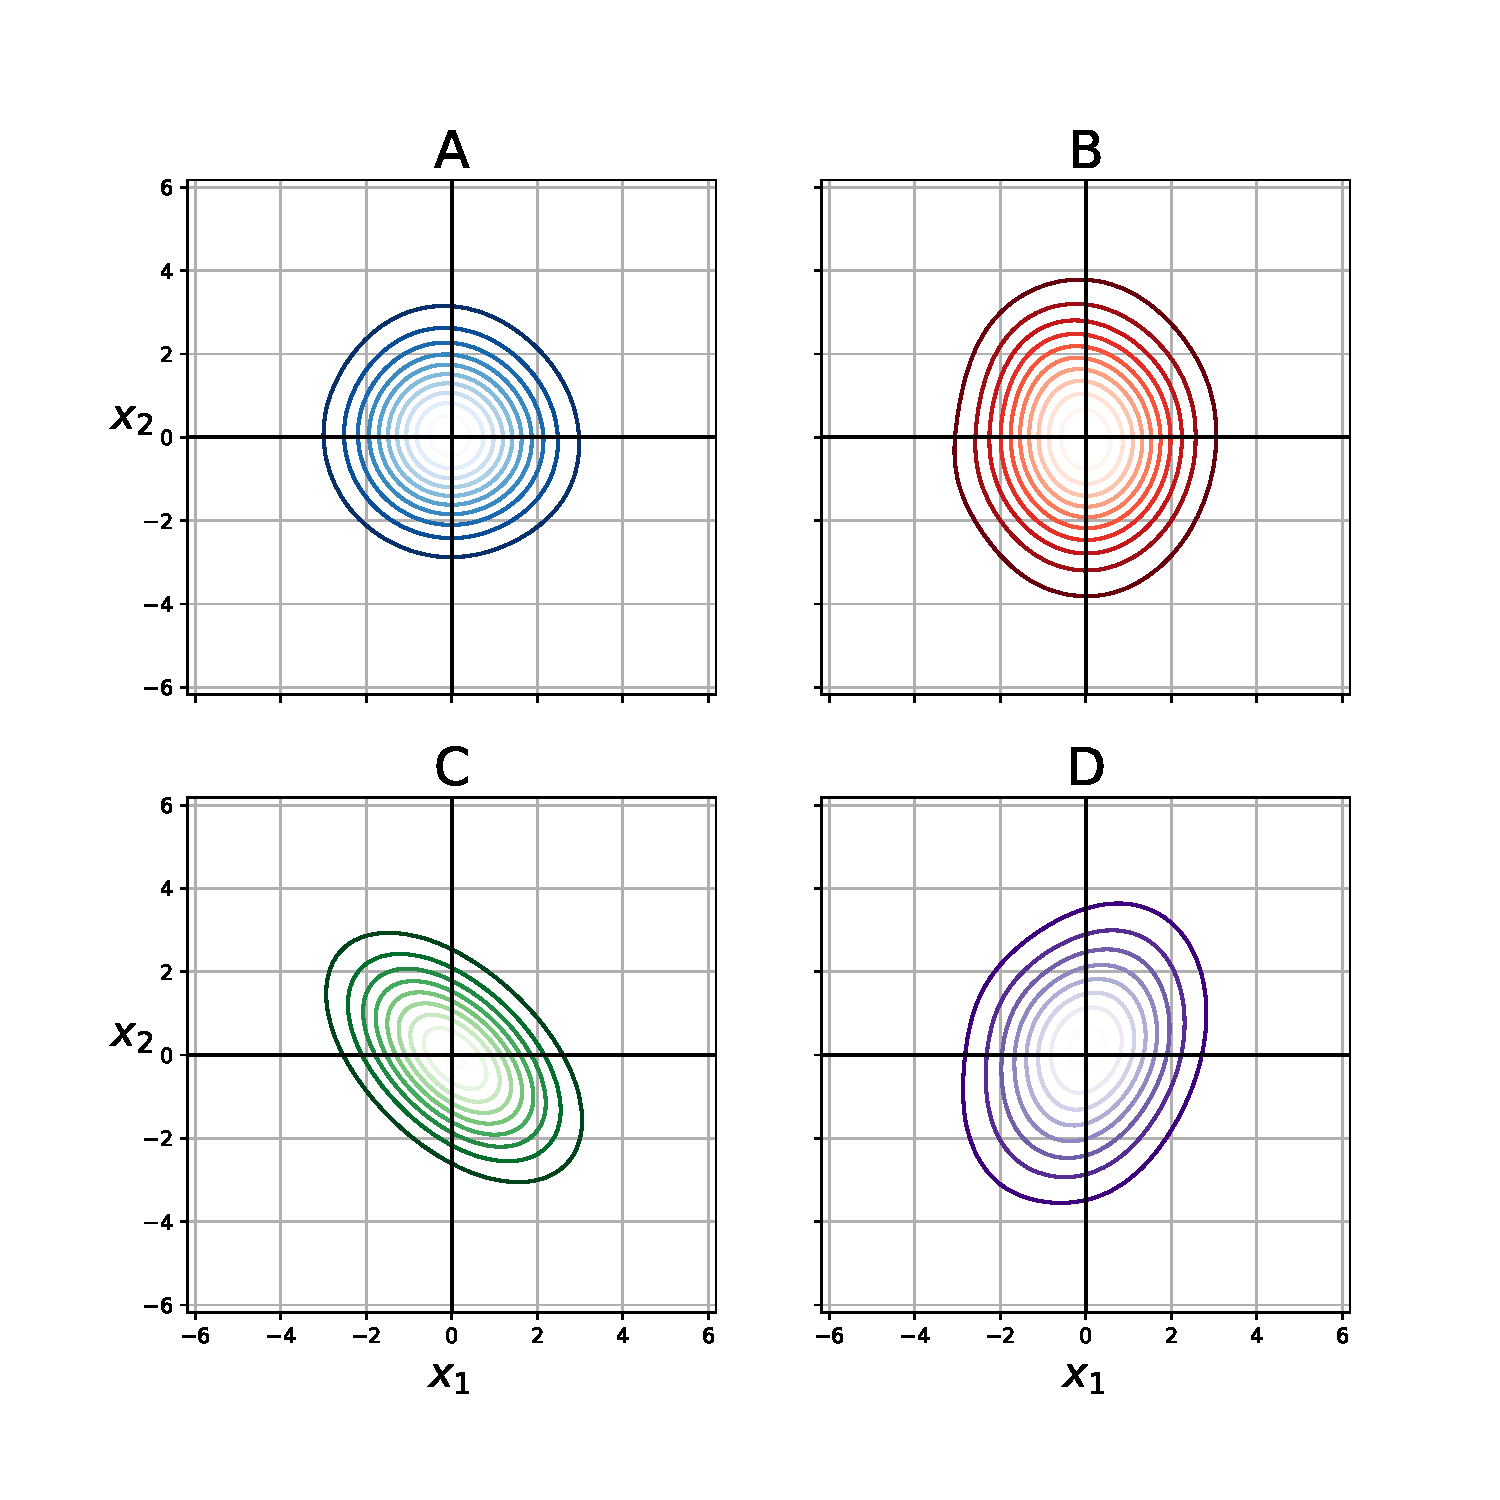
\includegraphics[width=0.99\textwidth]{img/cov}
         }
         \caption{Contour plots}
         \label{fig:linear}
     \end{subfigure}
\end{figure}
}

\question{Define a possible covariance matrix for each of the four datasets above.}

\mode<article>{

\begin{center}
\resizebox{.5\textwidth}{!}{%
\begin{tabular}{rl}
 ${\color{blue}\vec C_\mathrm{A} = \mat{1 & 0 \\ 0 & 1}}$ &  ${\color{red}\vec C_\mathrm{B} = \mat{1 & 0 \\ 0 & 2}}$\\[10mm]
 ${\color{darkgreen}\vec C_\mathrm{C} = \mat{1 & -1 \\ -1 & 1}}$ &  ${\color{byzantium}\vec C_\mathrm{D} = \mat{1 & 0.5 \\ 0.5 & 2}}$
\end{tabular}%
}
\end{center}
}



\end{frame}
